An off-axis parabolic mirror is a frequently used tool to focus an incoming collimated beam. It is made by cutting out a small section from a full parabolic mirror and thus it allows to deviate the beam path off the optical axis. Therefore, the focal point is at more accessible location and the target is not blocking the incoming collimated laser beam as in the case of a complete parabolic mirror. Obviously, the off-axis parabolic mirror is able to work reversibly, so it can take the light coming from a point source and produce a collimated beam. These physical properties make the off-axis parabolic mirror a valuable tool for many different optical purposes.

\floatsetup[figure]{style=plain, subcapbesideposition=top}
\begin{figure}[h!]
	\centering
	\sidesubfloat[]{{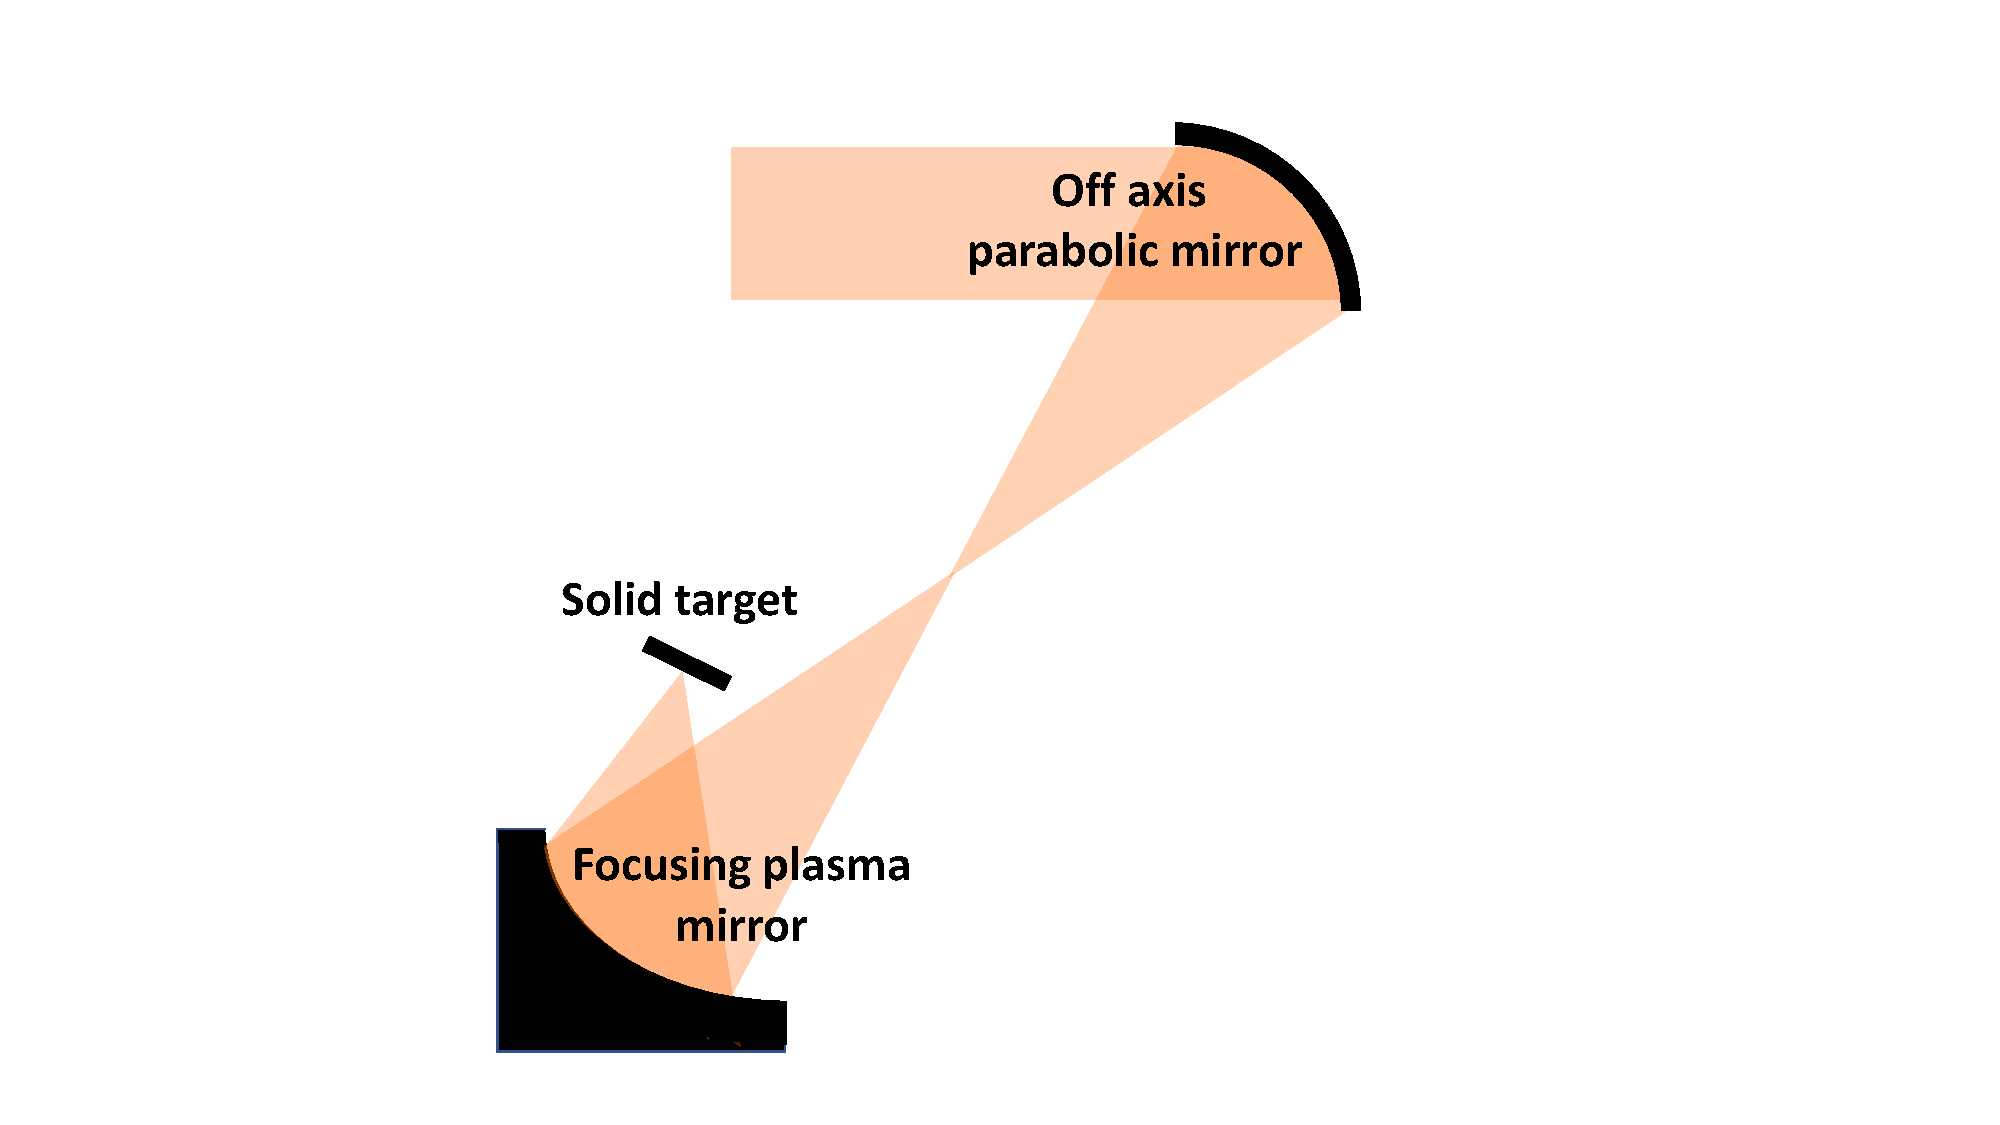
\includegraphics[width=0.35\linewidth]{./img/exp/diagram.pdf}}}
	\hspace{5mm}
	\sidesubfloat[]{{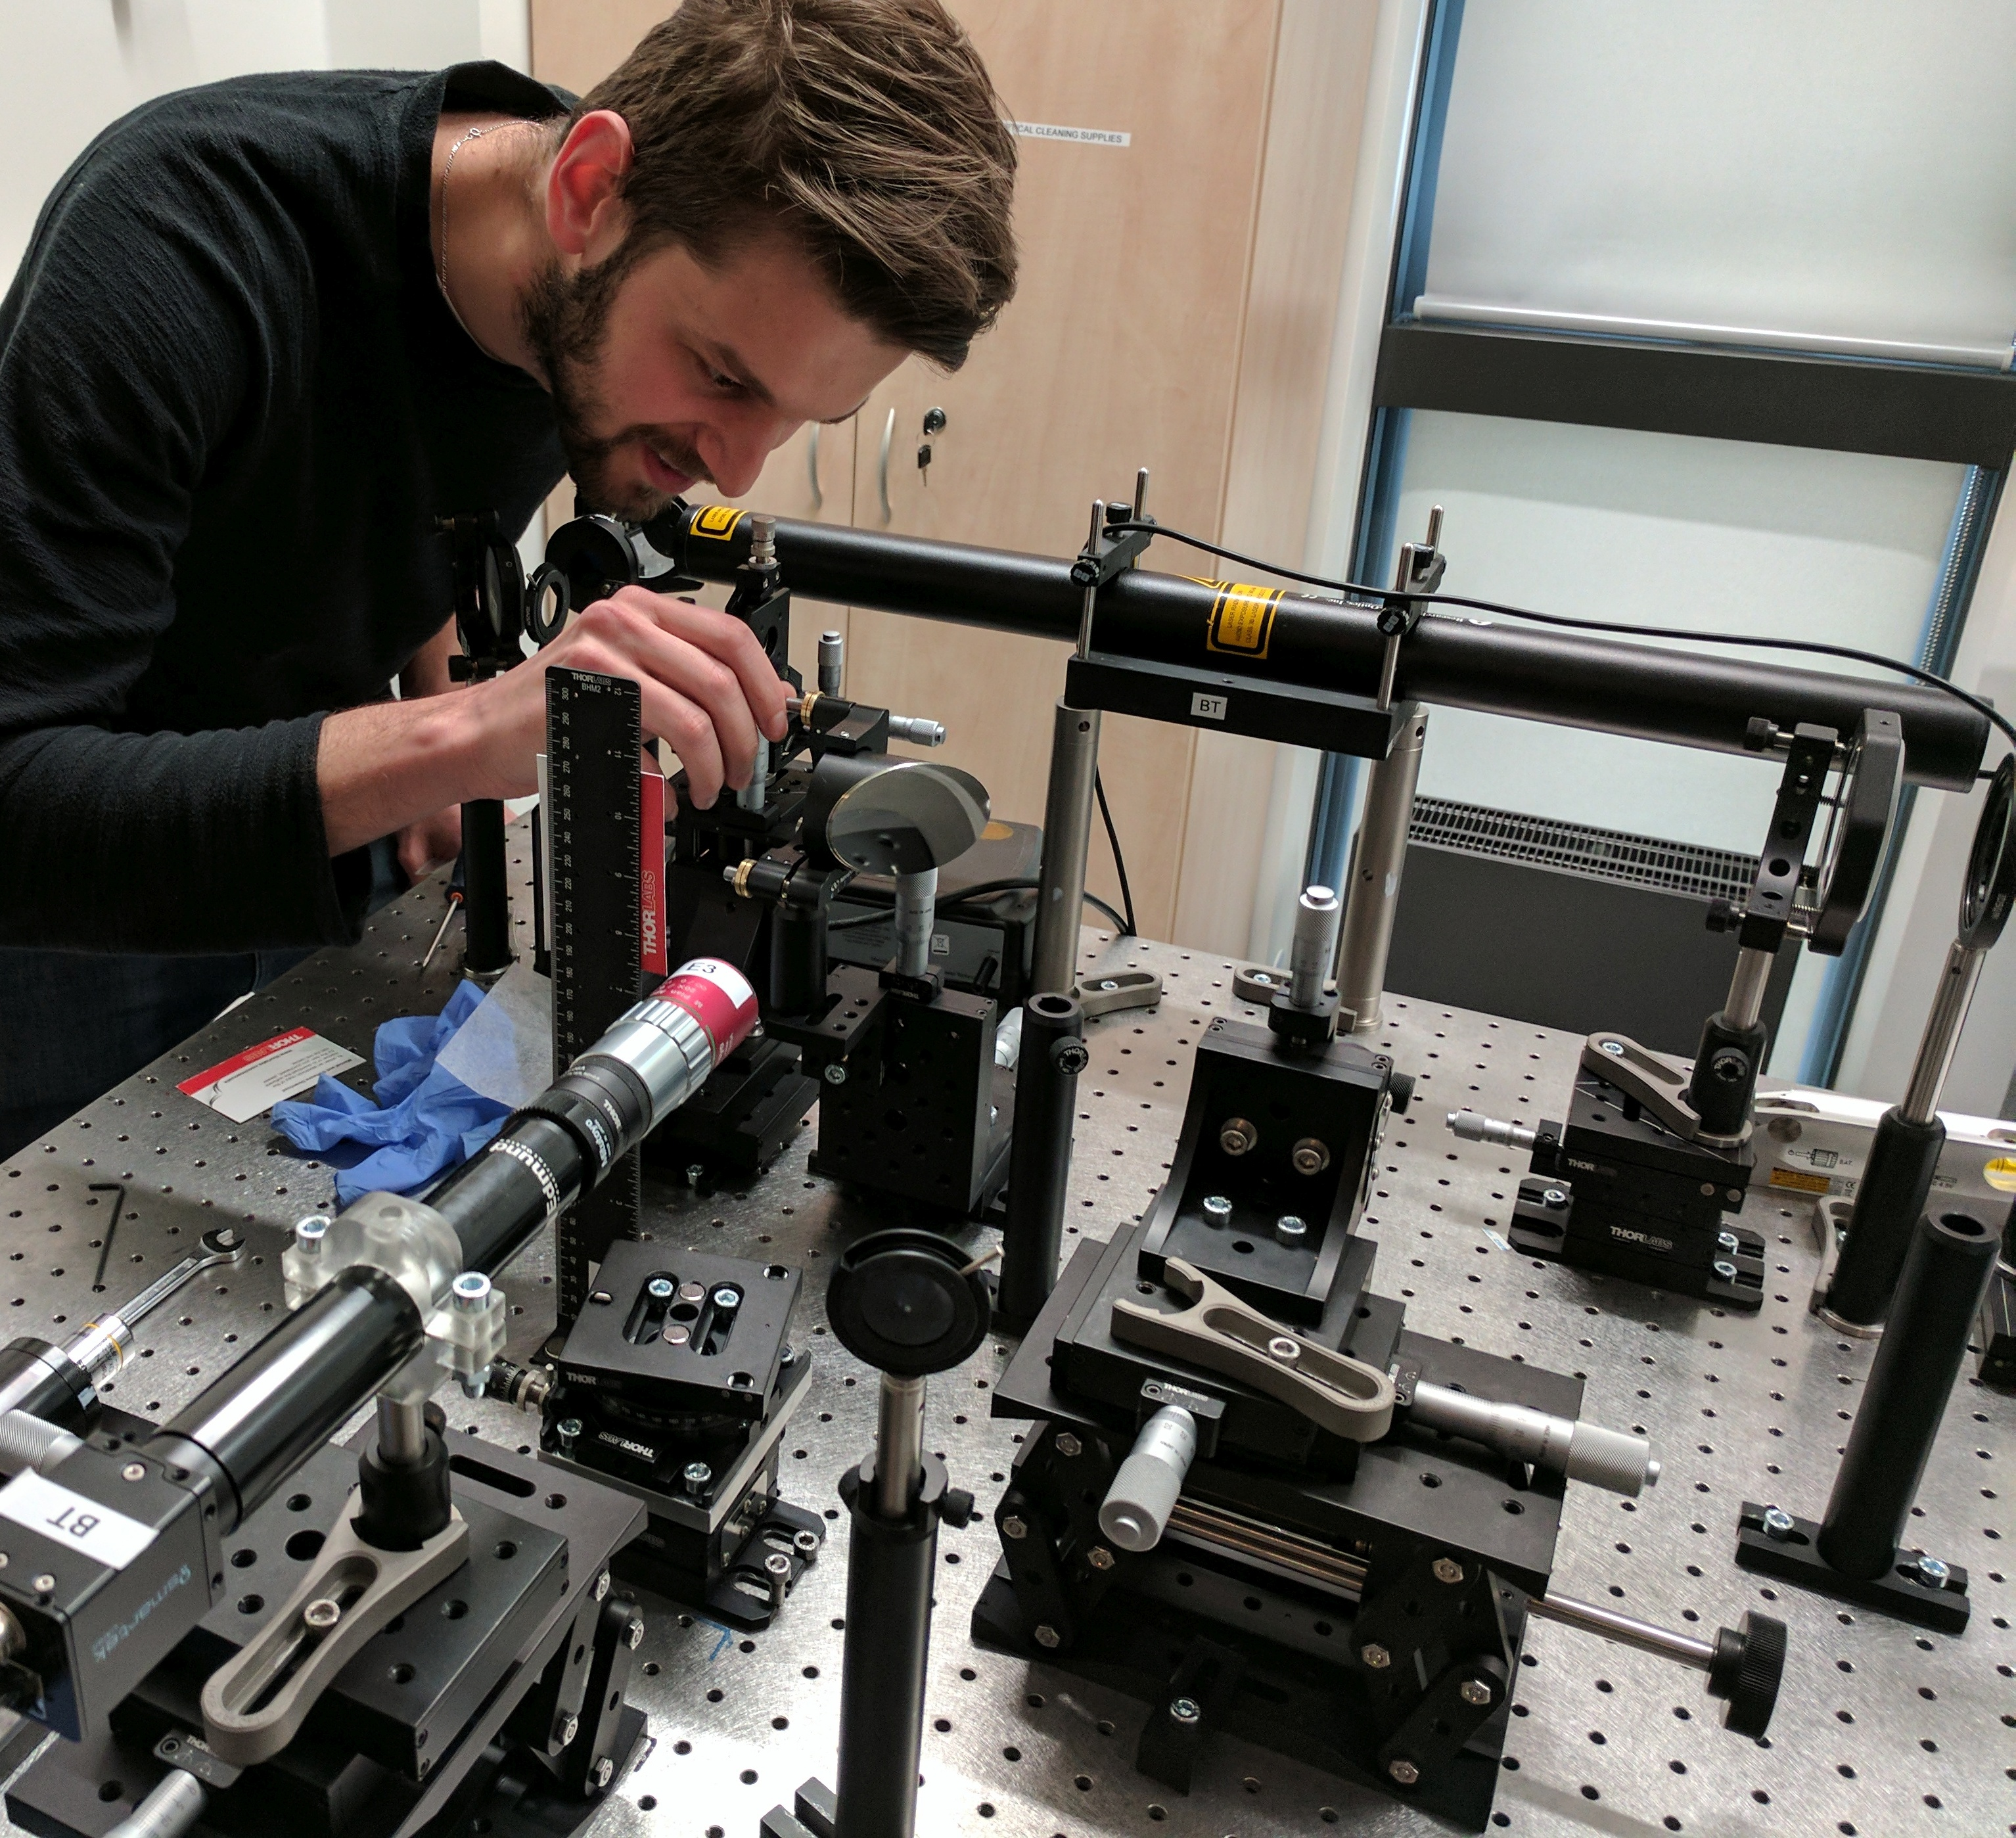
\includegraphics[width=0.4\linewidth]{./img/exp/photo2.jpg}}}
	\caption{\textbf{(a)} Schematic diagram showing the experimental set-up for tight-focusing. The incoming laser beam is focused by a conventional off-axis parabolic mirror to the first focal point of the ellipsoidal plasma mirror, beyond the light diverges and is reflected from the dense plasma created on the surface of plasma mirror. The beam is then imaged to the second focal spot where the target should be placed. \textbf{(b)} Photo taken at Extreme Light Infrastructure (ELI) laser facility capturing a very long and frustrating procedure of aligning an off-axis parabolic mirror.}
	\label{fig:9}
\end{figure}

However, as soon as the laser intensity exceeds $ 10^{13} \ \mathrm{W/cm}^{2} $, the surface of any material becomes strongly ionized. Therefore, in order to keep the energy density on the optical components below the damage threshold, the beam diameter has to be increased. This approach inherently imposes limits upon the geometrical characteristics of the focused beam such as the size of the focus. The focal spot can be alternatively decreased by implementing a small f-number focusing optic. However, since their focal length is inevitably very short and therefore they must be placed in close proximity to the interaction region, additional care has to be taken to protect the optical components because they can be easily damaged from debris induced by the exploded target flow. Note that such optics are typically very expensive.